\documentclass[10pt, a4paper, twocolumn]{article}

% ============================================================================
% Typography
% ============================================================================
\usepackage[T1]{fontenc}
\usepackage{mathpazo}           % Palatino text and math
\usepackage{microtype}          % Refined typography (tracking, kerning, spacing)

% ============================================================================
% Layout
% ============================================================================
\usepackage[margin=0.75in, columnsep=0.25in]{geometry}
\usepackage{setspace}
\singlespacing

% ============================================================================
% Figures and Tables
% ============================================================================
\usepackage{graphicx}
\usepackage{float}
\usepackage{booktabs}           % Professional tables
\usepackage{subcaption}         % Subfigures
\usepackage[font=small, labelfont=bf, labelsep=period]{caption}
\usepackage{placeins}           % For \FloatBarrier

% Graphics path
\graphicspath{{figures/}}

% Float parameters - keep figures near their text
\renewcommand{\topfraction}{0.9}
\renewcommand{\bottomfraction}{0.9}
\renewcommand{\textfraction}{0.1}
\renewcommand{\floatpagefraction}{0.7}
\setcounter{topnumber}{3}
\setcounter{bottomnumber}{3}
\setcounter{totalnumber}{5}

% ============================================================================
% Math and Science
% ============================================================================
\usepackage{amsmath}
\usepackage{amssymb}

% ============================================================================
% References and Links
% ============================================================================
\usepackage[numbers, sort&compress]{natbib}
\usepackage[colorlinks=true, linkcolor=black, citecolor=black, urlcolor=blue]{hyperref}

% ============================================================================
% Section Styling
% ============================================================================
\usepackage{titlesec}
\titleformat{\section}{\large\bfseries}{\thesection.}{0.5em}{}
\titleformat{\subsection}{\normalsize\bfseries}{\thesubsection.}{0.5em}{}
\titlespacing*{\section}{0pt}{1.5ex plus 0.5ex minus 0.2ex}{1ex plus 0.2ex}
\titlespacing*{\subsection}{0pt}{1ex plus 0.3ex minus 0.2ex}{0.5ex plus 0.1ex}

% ============================================================================
% Abstract Styling (for two-column layout)
% ============================================================================
\renewenvironment{abstract}{%
    \small
    \noindent\textbf{\abstractname.}
    \itshape
}{%
    \par\vspace{1em}
}

% ============================================================================
% Document Information
% ============================================================================
\title{\textbf{Slow Dynamics and High Variability in Clustered Networks}\\[0.5ex]
       \large Reproduction of Litwin-Kumar and Doiron (2012)}
\author{Arjun Puri\thanks{Berlin Center for Computational Neuroscience, alphabetical order} \and 
        Johan Kirikal\footnotemark[1] \and
        Shuo Wang\footnotemark[1]}
\date{\today}

% ============================================================================
% Document
% ============================================================================
\begin{document}

\twocolumn[
    \begin{@twocolumnfalse}
        \maketitle
        % ============================================================================
% Abstract
% ============================================================================
\begin{abstract}
    This report reproduces the key findings from Litwin-Kumar and Doiron
    (2012) on the slow dynamics and variability in clustered spiking
    networks. We implement their clustered network model and show that
    potentiated within-cluster connectivity introduces metastable firing
    states within the clusters. Using analyses from the original paper, we
    identify slow firing-rate fluctuations (via long-timescale decays in
    spike-count autocorrelation), higher trial-to-trial spike-count
    variability (via super-Poisson Fano Factors), and weak average pairwise
    correlations with a slightly elevated tail for within-cluster neurons.
    We also reproduce stimulus-quenched spiking variability. These results
    support the original paper's finding that clustered excitatory
    connections are sufficient to generate slow firing-rate fluctuations
    and stimulus-quenched variability in LIF networks---features also seen
    in cortical recordings.
\end{abstract}

        \vspace{1em}
    \end{@twocolumnfalse}
]

% ============================================================================
% Introduction
% ============================================================================
\section{Introduction}
\label{sec:introduction}

Cortical networks exhibit slow temporal dynamics and high trial-to-trial variability that are difficult to explain with classical balanced network models.

\subsection{Background}

The balance between excitation and inhibition is a fundamental organizing principle of cortical circuits.

\subsection{The Clustering Hypothesis}

Clustered connectivity within excitatory populations can generate slow dynamics through metastable attractor states.

\subsection{Objectives}

We aim to reproduce the core findings of the original study and explore extensions to the model.


% ============================================================================
% Results
% ============================================================================
\section{Results}
\label{sec:results}

We present our reproduction of the key findings from the original study.

\subsection{Metastable Dynamics in Clustered Networks}
\label{sec:metastable}

An excitatory-inhibitory (E/I) network with clustered E$\to$E connectivity
produces metastable ``high'' firing activity states within clusters that are
stable yet quick to transition. These high activity states persist for
hundreds of milliseconds to seconds before switching, leading to slow rate
dynamics and elevated trial-to-trial spike count variability (super-Poisson)
compared to unclustered networks.

\begin{figure}[t]
    \centering
    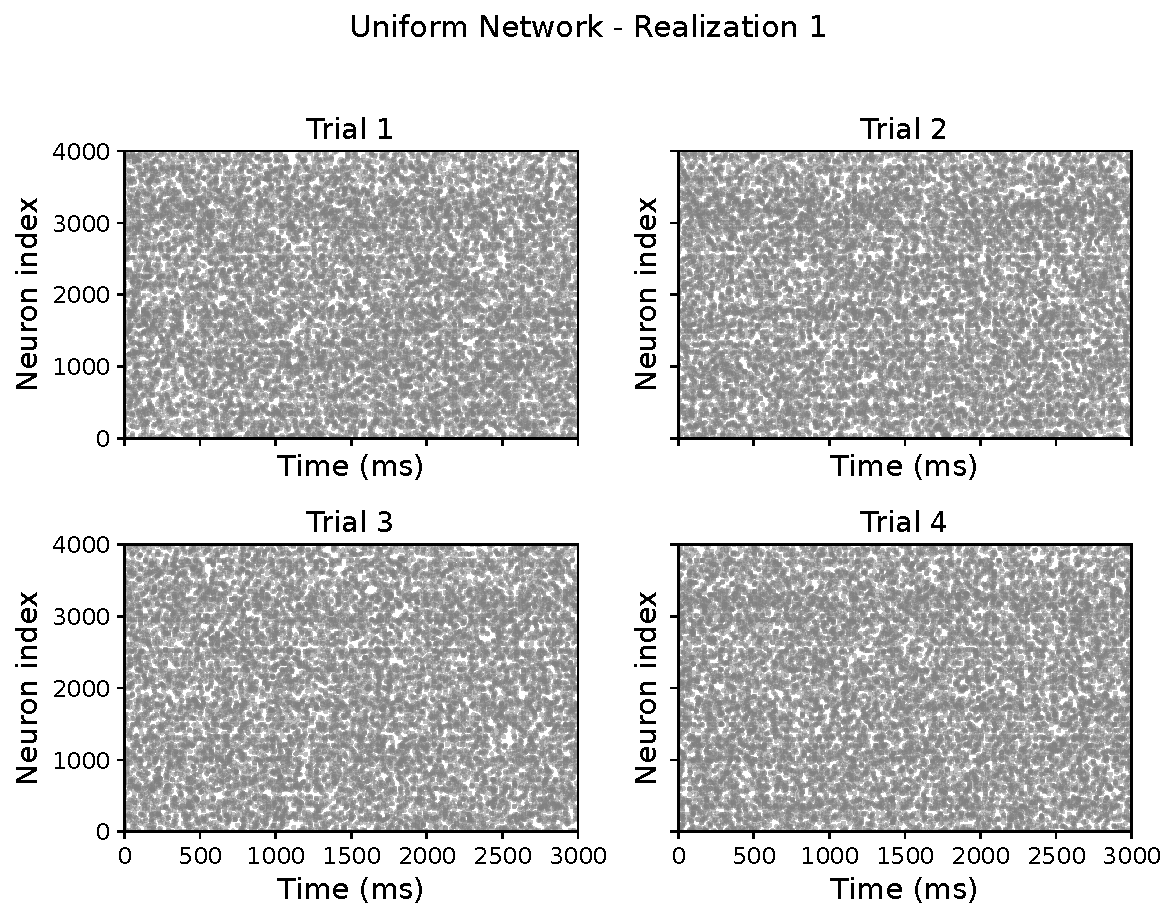
\includegraphics[width=\columnwidth]{rasters_uniform}
    \caption{Spike rasters from a uniform (unclustered) network across
    multiple trials.}
    \label{fig:rasters_uniform}
\end{figure}

\begin{figure}[t]
    \centering
    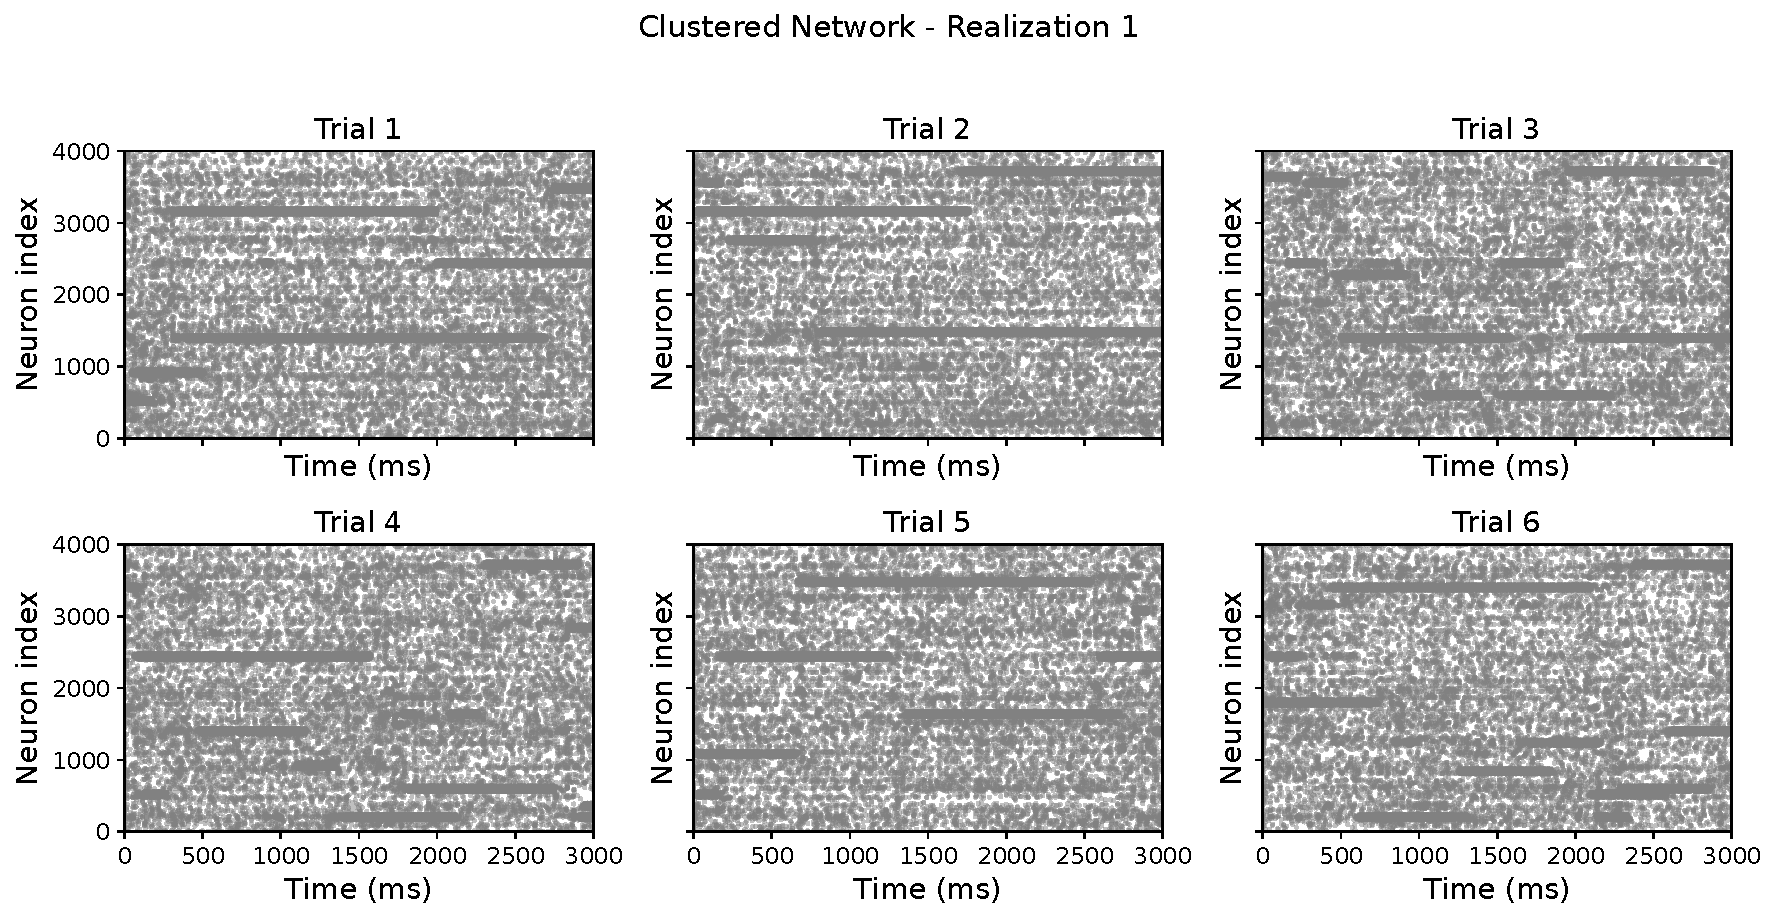
\includegraphics[width=\columnwidth]{rasters_clustered}
    \caption{Spike rasters from a clustered network across multiple trials.}
    \label{fig:rasters_clustered}
\end{figure}

\FloatBarrier
\subsubsection{Mean Rate}
\label{sec:mean_rate}

Despite the switching between high and low firing states, the clustered
network exhibits a low mean firing rate similar to that of the unstructured
network (Figure~\ref{fig:firing_rates}). This is likely due to additional
suppression within the network during high firing activity states. The high
activity epochs in clustered networks do not alter the overall mean firing
rate; however, the firing rate distribution broadens somewhat, likely
reflecting the alternation between high and low activity states.

\begin{figure}[t]
    \centering
    
\includegraphics[width=\columnwidth]{firing_rate_distribution}
    \caption{Distribution of firing rates for excitatory neurons in uniform
    and clustered networks. Both networks maintain low mean firing rates,
    though the clustered network shows a broader distribution reflecting
    the alternation between high and low activity states. Triangles indicate
    mean values.}
    \label{fig:firing_rates}
\end{figure}

\subsubsection{Variability}
\label{sec:variability}

Neurons in the clustered network exhibit Fano factors greater than one
(``super-Poisson'' spike count variability), as shown in
Figure~\ref{fig:fano_distribution}. Furthermore, the Fano factor increases
with the size of the counting window (Figure~\ref{fig:fano_vs_window}). This
pattern illustrates the presence of slow firing rate variability in clustered
networks---larger windows capture more of the slow rate fluctuations.

\begin{figure}[t]
    \centering
    
\includegraphics[width=\columnwidth]{fano_factor_distribution}
    \caption{Distribution of Fano factors across neurons for uniform and
    clustered networks. The clustered network exhibits a broader distribution
    with a higher mean (triangles), indicating greater spike count
    variability.}
    \label{fig:fano_distribution}
\end{figure}

\begin{figure}[t]
    \centering
    
\includegraphics[width=\columnwidth]{fano_factor_vs_window}
    \caption{Mean Fano factor as a function of counting window size. In the
    clustered network, the Fano factor increases with window size, reflecting
    slow rate fluctuations. The uniform network remains near the Poisson
    baseline (FF~=~1).}
    \label{fig:fano_vs_window}
\end{figure}

\FloatBarrier
\subsubsection{Correlations}
\label{sec:correlations}

Pairwise spike count correlations remain near zero on average for both
network types (Figure~\ref{fig:correlations_all}). However, in the clustered
network, within-cluster neuron pairs show a heavier positive tail in the
distribution of correlation coefficients (Figure~\ref{fig:correlations_cluster}).
This observation is consistent with the notion that clusters undergo
additional correlated firing rate transitions---switching between high and
low activity states---when examined across temporal windows spanning the
simulation. Furthermore, this positive tail becomes increasingly pronounced
as the counting window size increases (50~ms vs.\ 100~ms), as expected given
that within-cluster neurons share these slow rate fluctuations.

\begin{figure}[t]
    \centering
    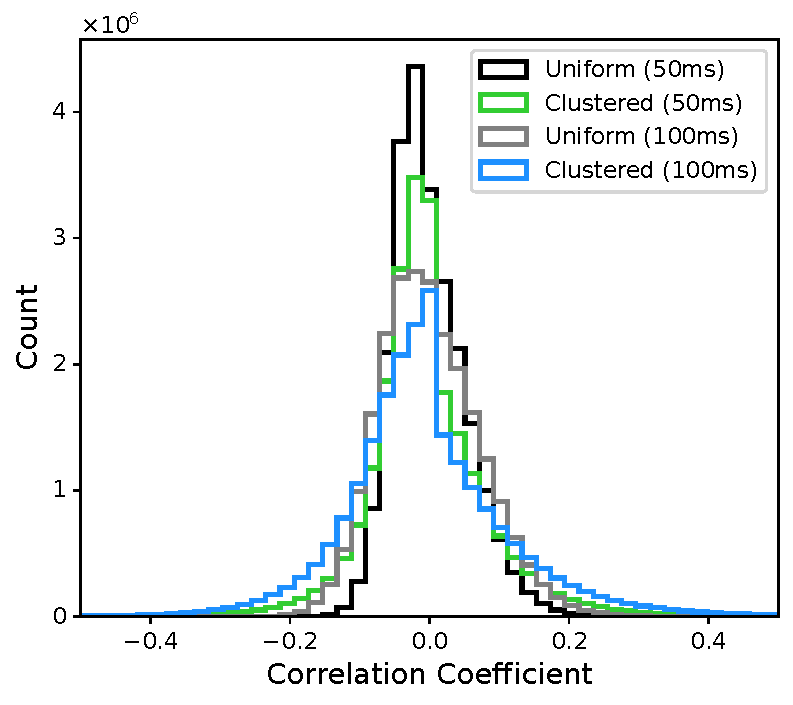
\includegraphics[width=\columnwidth]{correlation_all_pairs}
    \caption{Distribution of pairwise spike count correlations for all
    neuron pairs. Correlations remain centered near zero on average for
    both network types.}
    \label{fig:correlations_all}
\end{figure}

\begin{figure}[t]
    \centering
    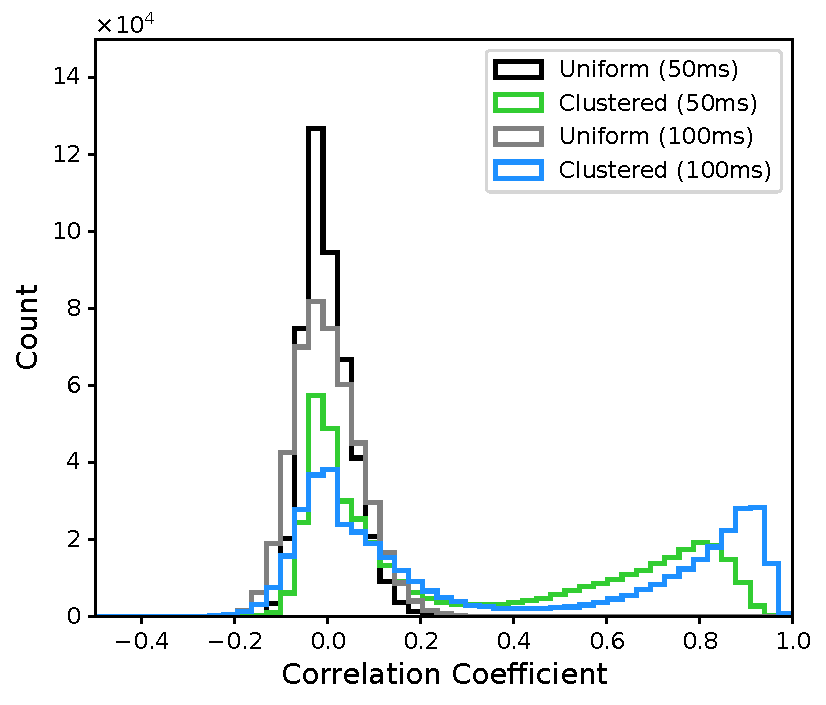
\includegraphics[width=\columnwidth]{correlation_same_cluster}
    \caption{Distribution of pairwise spike count correlations for
    within-cluster pairs only. The clustered network shows a heavy positive
    tail that increases with counting window size (50~ms vs.\ 100~ms).}
    \label{fig:correlations_cluster}
\end{figure}

\subsubsection{Timescales}
\label{sec:timescales}

Clustered networks exhibit substantially longer correlation times than
unstructured networks. The autocovariance function decays much more slowly
as a function of lag in clustered networks compared to their unstructured
counterparts. Similarly, the cross-covariance for within-cluster neuron
pairs decays slowly, indicating a shared correlated rate change among
neurons belonging to the same cluster.

% ============================================================================
% Critical Cluster Strength
% ============================================================================
\FloatBarrier
\subsection{Critical Cluster Strength}
\label{sec:critical_ree}

TODO

\begin{figure}[t]
    \centering
    
\includegraphics[width=\columnwidth]{fano_factor_vs_ree}
    \caption{Mean Fano factor as a function of cluster strength ($R_{EE}$).
    As within-cluster connection strength increases, the network transitions
    from Poisson-like variability to super-Poisson variability. The dashed
    line indicates the Poisson baseline (FF~=~1).}
    \label{fig:fano_vs_ree}
\end{figure}


% ============================================================================
% Discussion
% ============================================================================
\section{Discussion}
\label{sec:discussion}

The main goal of this project was to reproduce the paper by  Litwin-Kumar and Doiron (2012) \textcolor{red}{(add reference)}. Through replicating their results, we got our first experience in building a computational experimental model while working as a team. We acquired the key skills in doing neural network simulations using Brian2 and in converting the technical descriptions found in the original paper into actual code. In this process we also had to convert some key equations to a format more applicable to the Brian2 framework, since the paper Litwin-Kumar and Doiron (2012) \textcolor{red}{(add reference)} did not use Python.

To understand how successful our replication of the original paper was, Figure~\ref{fig:our_results} and Figure~\ref{fig:original_results} give us a comprehensive comparison between our work and the paper.

\begin{figure}[!htbp]
    \centering
    
\includegraphics[width=\columnwidth]{report/figures/our_results.png}
    \caption{The graphs combined together from our statistical analysis.}
    \label{fig:our_results}
\end{figure}

\begin{figure}[!htbp]
    \centering
    
\includegraphics[width=\columnwidth]{report/figures/original_results.jpg}
    \caption{Statistical analysis results from the original paper \textcolor{red}{(add reference).}}
    \label{fig:original_results}
\end{figure}

From this comparison, we see that most of the statistical analyses are very similar. The most fundamental difference is between Figure~\ref{fig:our_results} \textbf{(d)} and Figure~\ref{fig:original_results} \textbf{(d)}. From our experiment, the correlation coefficient figure displays a long heavy tail, with a significant bump around the 0.8 mark, while the original paper displayed a gradually diminishing positive tail, having almost no coefficients at 0.8.

While it is hard to know exactly the firing dynamics of the network in the original paper, we can still make a guess at the possible ex

% ============================================================================
% Extensions
% ============================================================================
\section{Extensions}
\label{sec:extensions}

Beyond reproduction, we explore extensions to the clustered network model.

\subsection{Extension 1}

Description of the first extension and its motivation.

\subsection{Extension 2}

Description of the second extension and its motivation.


% ============================================================================
% Model
% ============================================================================
\section{Model}
\label{sec:model}

We implement a recurrent spiking network with clustered excitatory connectivity using Brian2.

\subsection{Network Architecture}

The network consists of excitatory and inhibitory leaky integrate-and-fire neurons with structured connectivity.

\subsection{Neuron Model}

Membrane potential dynamics follow a leaky integrate-and-fire model with exponential synaptic filtering.

\subsection{Connectivity}

Connection probability between excitatory neurons depends on cluster membership, with enhanced within-cluster connectivity.

\subsection{Parameters}

Model parameters are chosen to match those of the original study.


% ============================================================================
% References
% ============================================================================
\bibliographystyle{plainnat}
\bibliography{references}

\end{document}
